\documentclass{article} 

\usepackage[numbers,sort&compress]{natbib} % citations
\usepackage{tikz} % diagrams
\usepackage{hyperref,url} % links

\begin{document}

\author{Elisa Schaeffer}
\date{\today}
\title{The structure of a manuscript in computational research}

\maketitle

\begin{abstract}
  Describe in present tense the nature and contributions of the
  present manuscript. Avoid citations and abbreviations as well as
  equations where possible.
\end{abstract}


\section{Introduction}
\label{int}

What is this about? What are you contributing? How is the rest of the
manuscript structured? What happens in Section \ref{bg}? How about
Sections \ref{met} and \ref{eval}? Also mention the nature of Section
\ref{conc}.

\section{Background}
\label{bg}

Relevant terminology and literature; all necessary definitions.  This
is where we could cite someone like \citet{elisa} if it were
relevant. You might also need equations like
\begin{equation}
  f(x) = a x + b,
\end{equation}
which is a line on a plane, $a$ being the slope and $b$ the intercept.

\section{Methodology}
\label{met}

This is where one explains what and how they do in their
research. There may be illustrations like that of Figure \ref{circle}
or data sets like Table \ref{data}. Pseudocode or links to program
code in
repositories\footnote{\url{https://github.com/SCS-Technology-and-Innovation/DDDM}}
may appear in this section. Note that you absolutely must refer to
every figure and table in the text and discuss them. They are not
decorations and you are {\bf not} to spend {\em any} time worrying
about their positioning within a page. Figures and tables go where they need to based on the template --- do not try to fix them in place.

\begin{figure}
  \begin{center}
    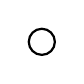
\begin{tikzpicture}[thick]
     \node[circle,draw] (c) at (0,0){};
    \end{tikzpicture}
  \end{center}
  \caption{All figures need to have a caption underneath that explains
    how to interpret them.}
  \label{circle}
\end{figure}

When making a table, always right-align (using \texttt{r}) any columns
that contain numerical information. For text and symbols, you can use
left (\texttt{l}) or center (\texttt{c}) alignment. If the table
contains paragraphs of text, use \texttt{p} and define the width (in
millimeters, for example) enclosed in curly braces right after that
\texttt{p}.

\begin{table}
  \caption{All tables also need a caption, but it goes above the content. You need to explain what the rows and the columns mean as well as any abbreviations, acronyms, symbols or notations used in the table content.}
  \label{data}
  \begin{center}
    \begin{tabular}{r|r|l} % three columns with different alignments and lines in between
      $x$ & $y$ & {\bf Class} \\
      10 & 19 & Regular \\
      -20 & 6 & Outlier
    \end{tabular}
  \end{center}
\end{table}

Remember to be clear, brief, and provide the right amount of detail
for your work to be understanable and reproducible.

\section{Evaluation}
\label{eval}

Explain how you have tested or assessed your proposed approach. What
was measured, when, how? Show and discuss your findings. You are
likely to use figures and tables again.

\section{Conclusions}
\label{conc}

First, in past tense, summarize the manuscript. Then highlight the
main contributions. Finally, describe possible future work that would
improve, generalize, or apply the present work (regardless of whether
or not you intend to carry out any of that yourself).

\bibliographystyle{plainnat}
\bibliography{refs}

\end{document}
